\documentclass[a4paper,12pt]{article} % тип документа

% Поля страниц
\usepackage[left=2.5cm,right=2.5cm,
    top=2cm,bottom=2cm,bindingoffset=0cm]{geometry}
    
%Пакет дял таблиц   
\usepackage{multirow} 
    
%Отступ после заголовка    
\usepackage{indentfirst}


% Рисунки
\usepackage{floatrow,graphicx,calc}
\usepackage{wrapfig}

% Создаёем новый разделитель
\DeclareFloatSeparators{mysep}{\hspace{1cm}}

% Ссылки?
\usepackage{hyperref}
\usepackage[rgb]{xcolor}
\hypersetup{				% Гиперссылки
    colorlinks=true,       	% false: ссылки в рамках
	urlcolor=blue          % на URL
}


%  Русский язык
\usepackage[T2A]{fontenc}			% кодировка
\usepackage[utf8]{inputenc}			% кодировка исходного текста
\usepackage[english,russian]{babel}	% локализация и переносы


% Математика
\usepackage{amsmath,amsfonts,amssymb,amsthm,mathtools, mathrsfs}


% Что-то 
\usepackage{wasysym}


\begin{document}
\begin{center}
	\footnotesize{ФЕДЕРАЛЬНОЕ ГОСУДАРСТВЕННОЕ АВТОНОМНОЕ ОБРАЗОВАТЕЛЬНОЕ 			УЧРЕЖДЕНИЕ ВЫСШЕГО ОБРАЗОВАНИЯ}\\
	\footnotesize{МОСКОВСКИЙ ФИЗИКО-ТЕХНИЧЕСКИЙ ИНСТИТУТ\\(НАЦИОНАЛЬНЫЙ 			ИССЛЕДОВАТЕЛЬСКИЙ УНИВЕРСИТЕТ)}\\
	\footnotesize{ФАКУЛЬТЕТ ОБЩЕЙ И ПРИКЛАДНОЙ ФИЗИКИ\\}
	\hfill \break
	\hfill\break
	\hfill\break
	\hfill \break
	\hfill \break
	\hfill \break
	\hfill \break
	\hfill \break
	\hfill \break
	\hfill \break
	\hfill \break
	\hfill \break
	\hfill \break
	\hfill \break
	\large{Лабораторная работа № 4.3.3\\\textbf{Исследование разрешающей способности микроскопа\\ методом Аббе}}\\
	\hfill \break
	\hfill \break
	\hfill \break
	\begin{flushright}
		Серебренников Даниил\\
		Группа Б02-826
	\end{flushright}
	\hfill \break
	\hfill \break
	\hfill \break
	\hfill \break
	\hfill \break
	\hfill \break
	\hfill \break
	\hfill \break
	\hfill \break
	\hfill \break
	\hfill \break
\end{center}
\begin{center}
	Долгопрудный, 2020 г.
\end{center}
\thispagestyle{empty}
\newpage

\textbf{Цель работы:} определение дифракционного предела разрешения объектива микроскопа методом Аббе.

\textbf{В работе используются:} лазер; кассета с набором сеток разного периода; линзы; щель с микрометрическим винтом; оптический стол с набором рейтеров и крепежных винтов; экран; линейка. 


\section{Теоретическая часть}
	\textit{Разрешающей способностью оптического прибора} называют минимальное расстояние $l_{\text{min}}$ между двумя точками в пространстве предметов, которое прибор может разрешить. Если наблюдения с помощью микроскопа ведутся при внешнем освещении, то, как правило, различные точки предмета рассеивают когерентные волны. Теория разрешающей способности для случая освещаемых объектов была разработана Аббе.

	Рассмотрим когерентно освещенный объект, наблюдаемый в объектив микроскопа. Минимальное разрешаемое объективом расстояние определяется условием
	\begin{equation}
		\label{min}
		l_{\text{min}} \approx \frac{\lambda}{\sin A} \approx \frac{\lambda}{D/2f},
	\end{equation}
	где $A$ -- апертурный угол микроскопа, $D$ -- диаметр диафрагмы. При этом диафрагма, расположенная симетрично, пропускает нулевой и $\pm 1$ дифракционные максимумы.
	
	В нашей работе применяется двумерная решётка -- сетка. В таком случае главные максимумы возникают тогда, когда одновременно выполняются условия:
	\begin{equation}
		\label{system}
		\begin{cases}
			d \sin \theta_x = m_x \lambda, \\
			d \sin \theta_y = m_y \lambda,
		\end{cases}
	\end{equation}
	где $m_x$ и $m_y$ -- целые числа, харакетризующие порядки дифракционных максимумов, $\theta_x$ и $\theta_y$ -- направления нв главные дифракционные максимумы в горизонтальное и вертикальной плоскостях соответственно.
	
	Максимумы, удовлетворяющие условию $\theta_x, \theta_y < A$, создают в задней фокальной плоскости $F$ объектива картину дифракции Фраунгофера (рис.~\ref{ris:max}) -- первичное изображение.
	\begin{figure}[H]
		\center{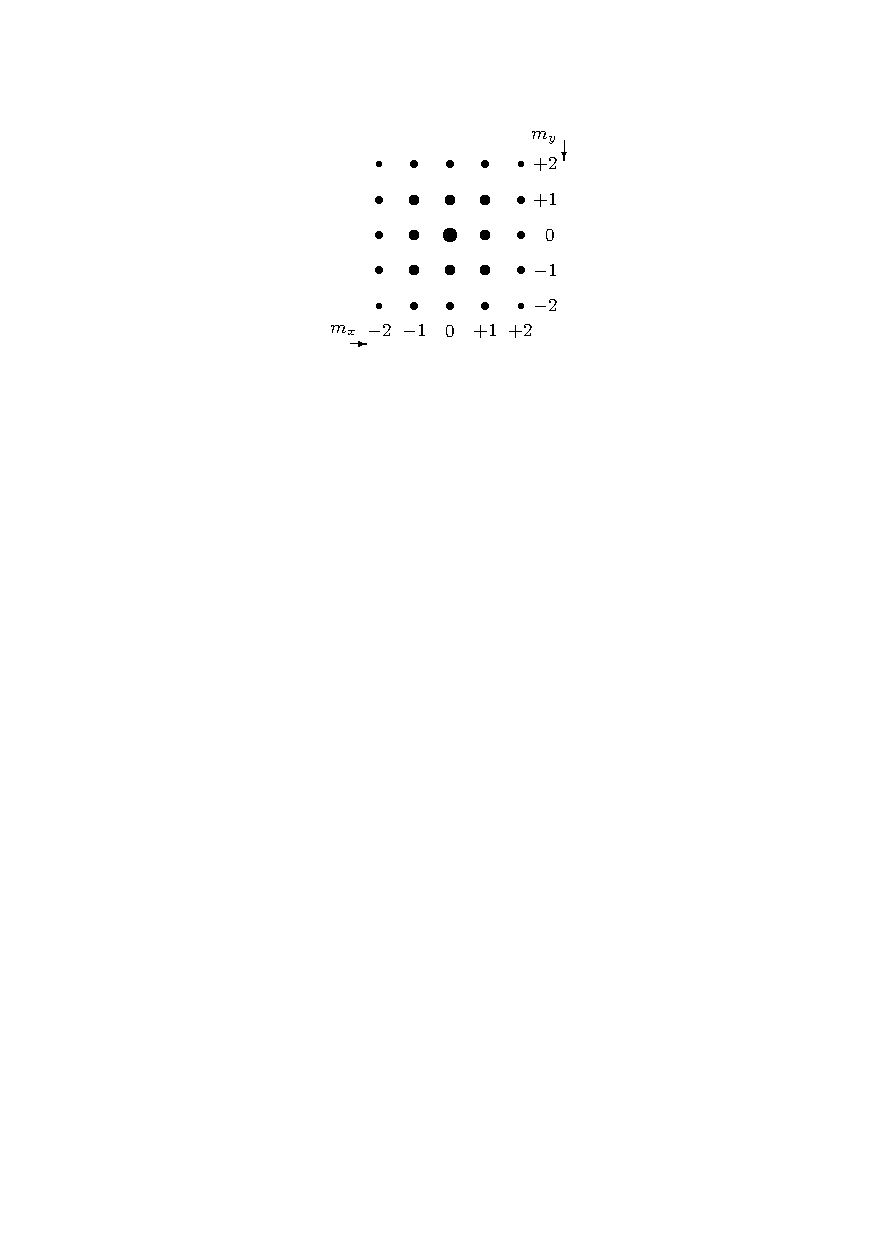
\includegraphics[scale=1.0]{max.pdf}}
		\caption{Дифракция Фраунгофера на двумерной решётке (сетке). Максимумы изображены кружками, размеры которых характеризуют интенсивности.}
		\label{ris:max}
	\end{figure}
	
	Если теперь поместить в фокальной плоскости щель так, чтобы через неё проходили дифракционные максимумы с $m_x = 0$ и $m_y =0, \pm 1, \pm 2, ...$ (с $m_y = 0$ и $m_x =0, \pm 1, \pm 2, ...$), то в плоскости $P_2$ получится изображение решётки с горизонтальными (вертикальными) штрихами. Таким образом можно продемонстрировать явление \textit{пространственной фильтрации} -- выделение различных структур в изображении.
	\newpage
\section{Экспериментальная установка}
	Схема модели проекционного микроскопа приведена на рис.~\ref{ris:ustanovka}. Предметом служат сетки, расположенные в кассете. Смена сеток осуществляется поворотом внешнего кольца кассеты.
	\begin{figure}[H]
		\center{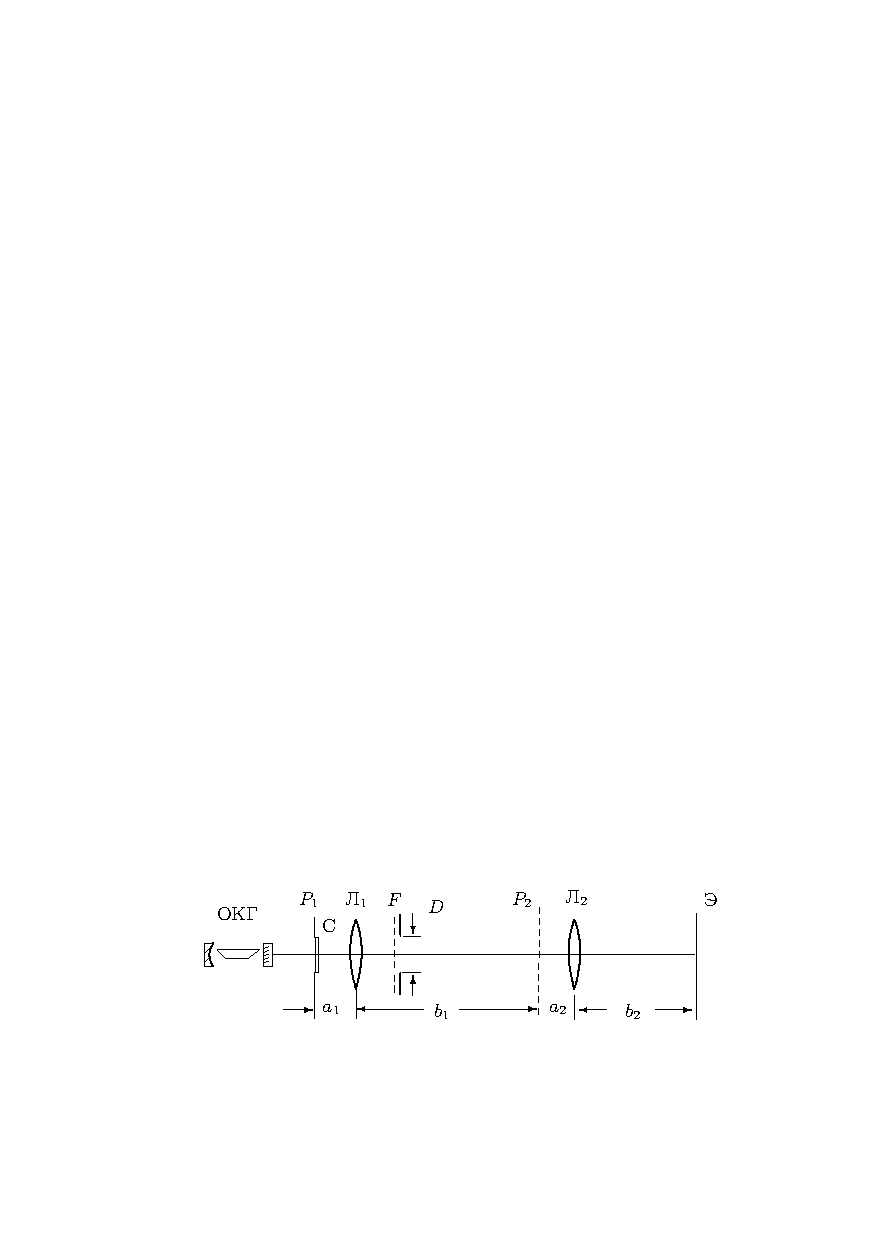
\includegraphics[scale=1.0]{ustanovka.pdf}}
		\caption{Схема экспериментальной установки -- модель проекционного микроскопа.}
		\label{ris:ustanovka}
	\end{figure}
	Изображение сетки периодически повторяется -- \textit{репродуцируется} -- в пространстве между сеткой и первой линзой. Для выделения геометрического изображения среди множества репродуцированных изображений сетки на одну из сеток наложена тонкая проволока, то есть непереодический объект, изображение которого не репродуцируется.
	
\section{Ход работы}
	\begin{enumerate}
		\item
			Определение периода решёток по их пространственному спектру
		\item 
			Определение периода решёток по изображению, увеличенному с помощью модели микроскопа
		\item
			Определение периодов решёток по оценке разрешающей способности микроскопа
		\item 
			Наблюдение явлений пространственной фильтрации и мультиплицирования.
	\end{enumerate}
\newpage
\section{Экспериментальные данные}

	Измерим расстояние $L = 140$ см от сетки до экрана и определим периоды решёток по их пространственному спектру. Для этого из формулы (\ref{system}) выразим $d = m \lambda / \sin \theta$, причем $\sin \theta \approx (l/n)/L$ и $m = 1$, где $l$ -- расстояние между удалёнными друг от друга максимумами. Используемый нами лазер имеет длину волны $\lambda = 532$ нм.
	
	\floatsetup[table]{capposition=top}	
	\begin{table}[H]
		\caption{Результаты измерений 1 способом.}
		\label{table:exp1}
		\begin{tabular}{|c|c|c|c|c|c|}
			\hline
			$N$      & 1     & 2     & 3     & 4      & 5      \\ \hline
			$n$      & 1     & 1     & 3     & 5      & 6      \\ \hline
			$l$, мм  & 38    & 27    & 39    & 32     & 29     \\ \hline
			$d$, мкм & 19,6 & 27,6 & 57,3 & 116 & 154 \\ \hline
		\end{tabular}
	\end{table}
	
	Измерим расстояния $a_1 = 145$ мм, $b_1+a_2 = 655$ мм, $b_2 = 1200$ мм, $a_2 \approx f_2 = 25$~мм, $f_1 = 110$ мм и определим периоды решёток по изображеннию, увеличенному с помощью микроскопа по очевидной формуле $d = (l/n)/\Gamma$, где $\Gamma = \frac{b_1b_2}{a_1a_2} = 209$ -- увеличение для оптической системы.
	\floatsetup[table]{capposition=top}	
	\begin{table}[H]
		\caption{Результаты измерений 2 способом.}
		\label{table:exp2}
		\begin{tabular}{|c|c|c|c|c|c|}
			\hline
			$N$      & 1    & 2     & 3    & 4    & 5   \\ \hline
			$n$      & 20   & 10    & 10   & 5    & 5   \\ \hline
			$l$, мм  & 52   & 40    & 77   & 80   & 105 \\ \hline
			$d$, мкм & 12,5 & 19,14 & 36,8 & 76,6 & 100 \\ \hline
		\end{tabular}
	\end{table}

	Определим для каждой решётки минимальный размер диафрагмы $D$, при котором на экране ещё видно изображение сетки. Из формулы~(\ref{min}) следует, что $d =~2\lambda f_1 / D$.

	\floatsetup[table]{capposition=top}	
	\begin{table}[H]
		\caption{Результаты измерений 3 способом.}
		\label{table:exp3}
		\begin{tabular}{|c|c|c|c|}
			\hline
			$N$      & 3    & 4   & 5   \\ \hline
			$D$, мкм & 1660 & 840 & 510 \\ \hline
			$d$, мкм & 70,5 & 139 & 229 \\ \hline
		\end{tabular}
	\end{table}

	
	Сравним результаты рассчетов периодов решёток разными способами.
	
	\floatsetup[table]{capposition=top}	
	\begin{table}[H]
		\caption{Сравнение результатов.}
		\label{table:compare}
		\begin{tabular}{|c|c|c|c|c|c|}
			\hline
			$N$        & 1    & 2     & 3    & 4    & 5   \\ \hline
			$d_1$, мкм & 19,6 & 27,6  & 57,3 & 116  & 154 \\ \hline
			$d_2$, мкм & 12,5 & 19,14 & 36,8 & 76,6 & 100 \\ \hline
			$d_3$, мкм & --   & --    & 70,5 & 139  & 229 \\ \hline
		\end{tabular}
	\end{table}
		
		
\newpage
\section {Обработка результатов}
	Для проверки теории аббе построим график зависимости $d = d(1/D)$, взяв периоды сеток, определенные по спектру.
	
	\floatsetup[table]{capposition=top}	
	\begin{table}[H]
		\caption{Данные для построения $d=d\,(1/D)$.}
		\label{table:d=d(1/D)}
		\begin{tabular}{|c|c|c|c|}
			\hline
			$N$              & 3     & 4    & 5    \\ \hline
			$1/D$, нм$^{-1}$ & 0,602 & 1,05 & 1,96 \\ \hline
			$d$, мкм         & 57,3  & 116  & 154  \\ \hline
		\end{tabular}
	\end{table}
	
	
	\begin{figure}[H]
		\center{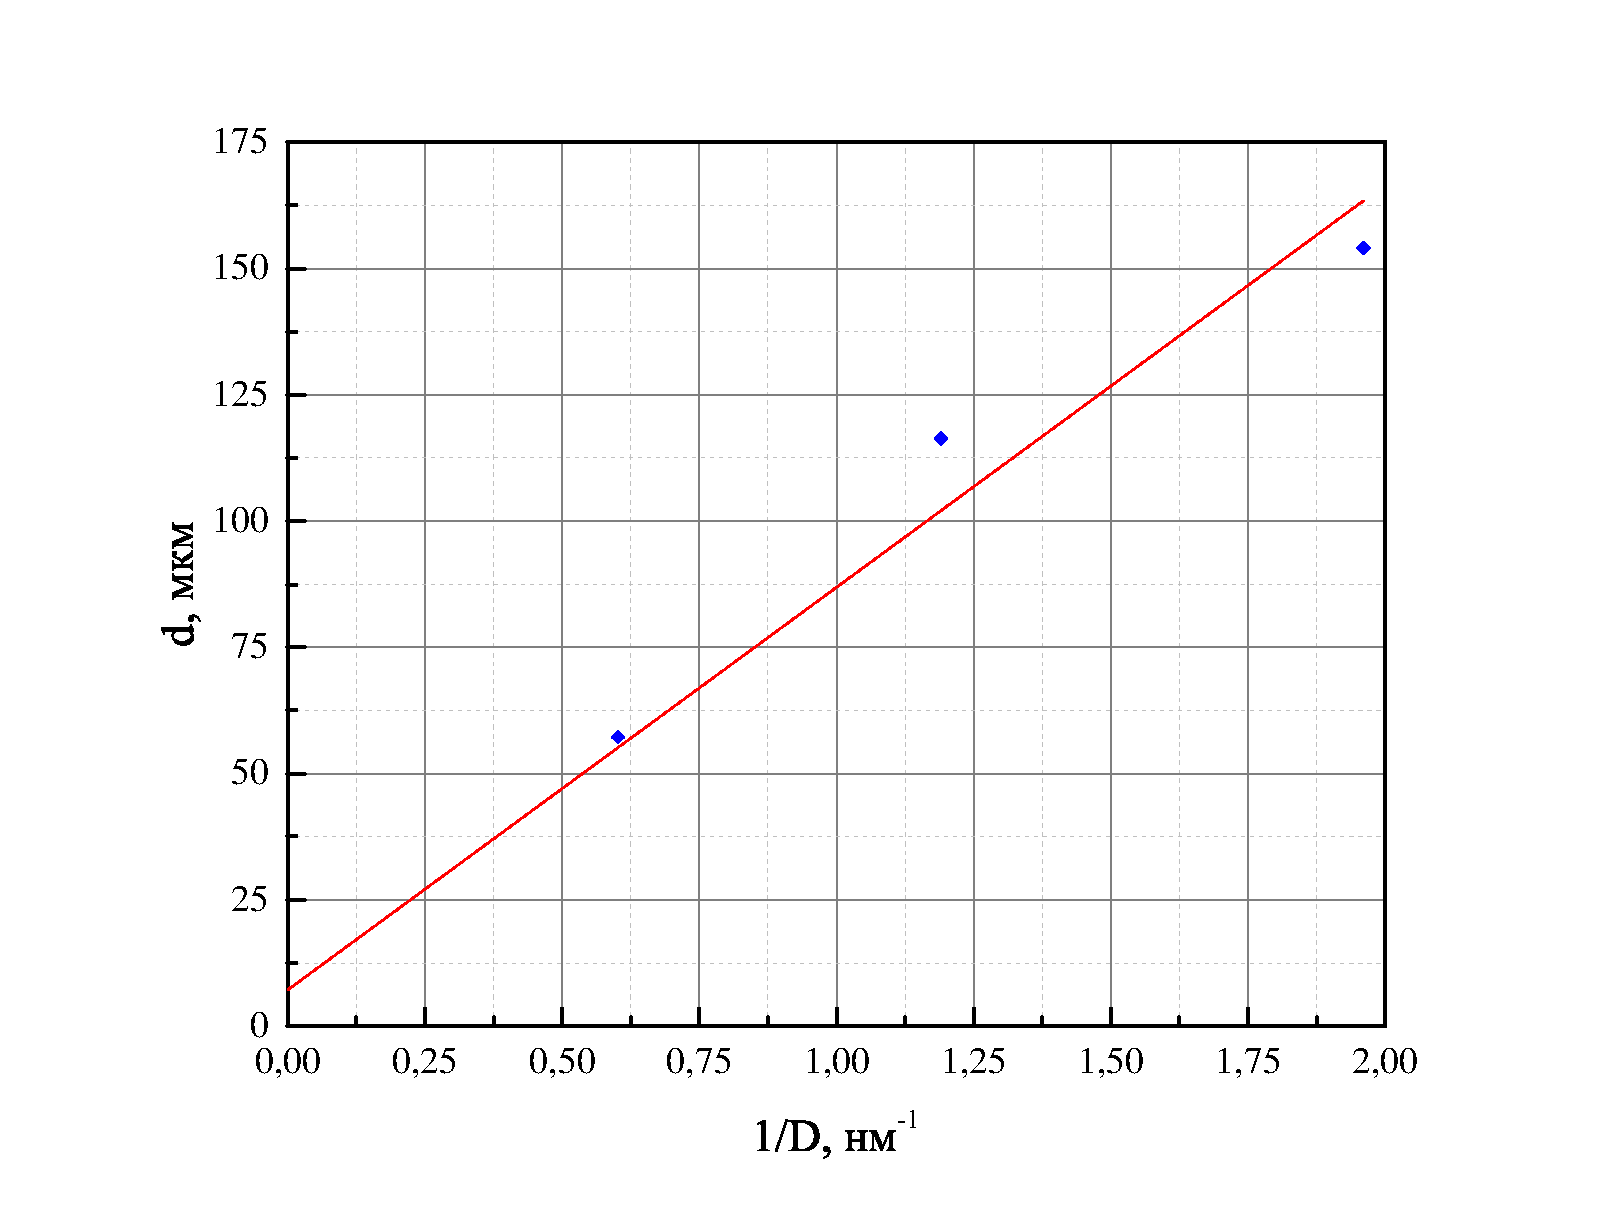
\includegraphics[scale=0.4]{graph.pdf}}
		\caption{Зависимость $d=d\,(1/D)$.}
		\label{ris:d=d(1/D)}
	\end{figure}


\section {Обсуждение результатов}
	В ходе данной лабораторной работы мы определили периоды дифракционных решёток различными способами (табл.~\ref{table:compare}). Полученные результаты отличаются друг от друга существуенно (наименьший от наибольшего в два раза), хотя имеют одинаковый порядок величины. Это может быть связано с приближенным характером используемой теории, неточностью определения величин $a_2$ и $b_1$, неисправностью источника света, который в ходе выполнения лабораторной работы периодически выключался. 
	
	Стоит отметить, что у всех величин, полученных прямым измерением, мы принебрегли случайной погрешностью, так как она мала по сравнению с систематической, которая явным образом повлияла на разброс результатов.
	
	Не смотря на расхождения, нам удалось убедиться в справедливости формулы~(\ref{min}), то есть проверка теории Аббе оказалась положительной. Действительно, периоды решёток, определенные в первом и третьем способах, отличаются от их среднего значения на 20 \%, что может навести на мысль о том, что во втором способе, скорее всего, имеется грубая ошибка и эксперимент требует повторного проведения.
	
	Выход из строя источника света не позволил пронаблюдать за явлениями фильтрации и мультиплицирования.
	
\newpage	
\section{Выводы}
	\begin{enumerate}
		\item 
			Вычислили периоды решёток различными способами;
		\item 
			Метод Аббе по определению дифракционного предела разрешения объектива микроскопа даёт верные результаты.
		
	\end{enumerate}


\end{document}